\documentclass[11pt]{article}
\usepackage{../EllioStyle}
\usepackage{graphicx}

\title{Homework 6}
\author{Elliott Pryor \\
Collaborated with: Nathan Stouffer}
\date{22 April 2021}

\rhead{Homework 6}
\lhead{Elliott Pryor}

\graphicspath{{./}{images/}}


\newcommand{\A}{{\mathcal{A}}}

\makeatletter
\def\mathcolor#1#{\@mathcolor{#1}}
\def\@mathcolor#1#2#3{%
  \protect\leavevmode
  \begingroup
    \color#1{#2}#3%
  \endgroup
}
\makeatother


\algdef{SE}[DOWHILE]{Do}{doWhile}{\algorithmicdo}[1]{\algorithmicwhile\ #1}

\begin{document}

\maketitle

This homework assignment occurs at the same time as the course project.  These
questions should take substantially less time then the first five assignments.
While I invite you to spend as much time on these problems as you like, I do not
expect you to spend any more than 3 hours on the entire assignment so that you
can focus on your projects.


\problem{1}

We saw in class that the Voronoi diagram of a set of points in $\reals^2$ is the
projection of the upper envelope of the dual lifted set of planes in $\reals^3$.
What does the projection of the lower envelope correspond to? Similarly, what
does the projection of the upper convex hull of the points lifted to $\reals^3$
correspond to?

You MAY (but do not need to) answer these questions by researching on the
internet. Cite the sources you were using and give an explanation in your own
words

\hrule

I think that the projection of the lower envelope is the convex hull.
Or more specifically, the projection is the voronoi diagram of the points making up the convex hull.
This projection is flipped/mirrored somehow that I can't really visualize, but the 
planes on the lower envelope correspond to points on the convex hull.
At a high level: points on the convex hull are the furthest out (there is a halfplane through
the point dividing the plane where all points are on LHS of plane). 
Since they are the furthest out they will have the most extreme slope (in some direction)
thus far enough along that direction the plane is below all other planes and is thus on the lower envelope.



The upper convex hull of the lifted points is the delauney triangulation of the points
on the convex hull. Similar as before, these points are the most extreme, and are the highest up. 
So they will be on the convex hull. 
Consider the example of a ton of points within radius 0.5 of the origin and points at (1,1), (-1,-1)
(0.9, -1), (-1, 0.9). The upper convex hull is a house roof shaped thing. And it forms
two triangles which is the delauney triangulation of these points.











\problem{2}

We saw in class how to solve motion planning problems in $\reals^2$ in a static
environment of polygonal obstacles by computing the configuration space with
Minkowski sums.  While theoretically interesting, often, explicitly computing
the configuration space is too computationally intensive.  Describe another
method for performing motion planning.

You MAY (but do not need to) answer this question by researching on the
internet. Cite the sources you were using and give an explanation in your own
words

\hrule

Similar to what I had partially mentioned in class with going to tangent points. 
We draw line s-t. We slide the robot along the line until we hit a shape (more on computing this in a bit).
(we assume robot can't spin/rotate only translate). 
So if s-t line intersects a polygon. We draw line $\ell$ from s to the tangent point of this polygon.
Sliding the robot along this line continuously and checking for intersection is the same as
taking a vertex of the robot and making it a line segment parallel to $\ell$.
We check if/where this segment intersects an obstacle. We move to there 
and slide the robot in the direction of the edge that we intersected until this vertex no longer intersects
the edge that we hit. We repeat.
We also need to take the vertices of obstacles and make them lines to check for when a point
of an obstacle hits the edge of robot (not edge of robot hits obstacle).


\begin{figure}[h]
    \centering
    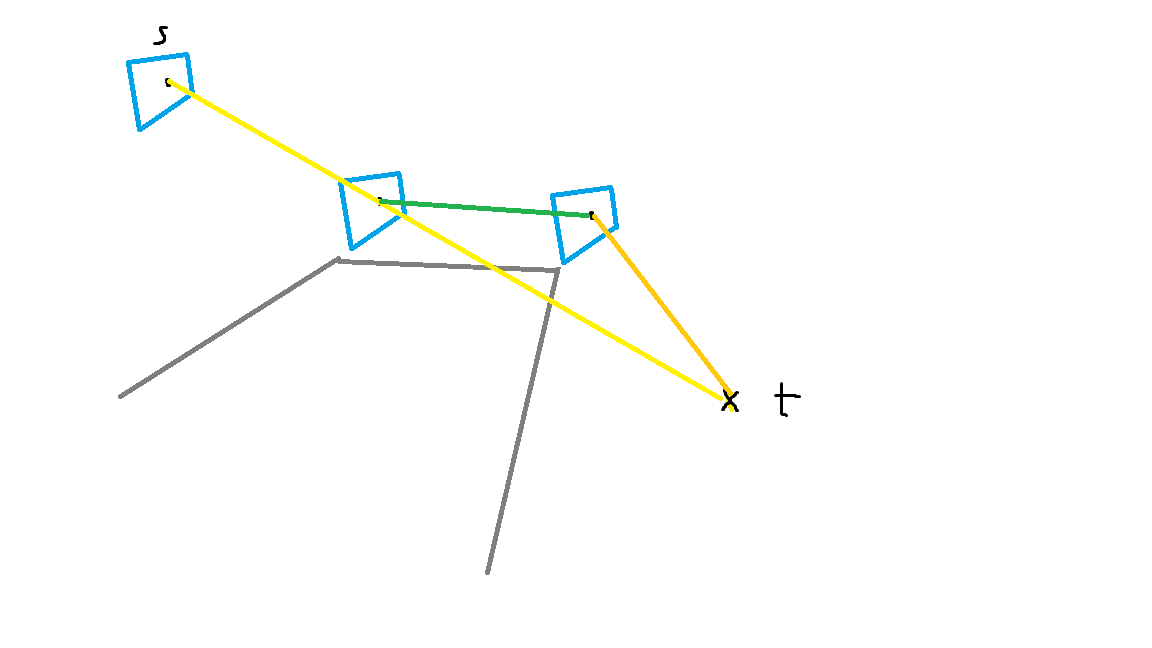
\includegraphics[scale = 0.5]{problem2.png}
    \caption{Problem 2 drawing basic idea }
\end{figure}





\problem{3}

Consider an arrangement $\A$ of six lines $\ell_1, \ell_2, \ldots, \ell_6$ and
let $f$ be an arbitrary vertex, edge, or face of $\A$. Then $f$ has an
associated sign vector $(s_1, s_2, s_3, s_4, s_5, s_6)$, where for each $1 \le i
\le 6$:

$$
    s_i =
    \begin{cases}
        +1, & \text{if $f$ lies above $l_i$} \\
        0,  & \text{if $f$ lies on $l_i$} \\
        -1, & \text{if $f$ lies below $l_i$}
    \end{cases}
$$

\begin{enumerate}

    \item For each of the sign vectors below, give an arrangement of six lines
        that has a vertex, edge, or face with this sign vector. Label the lines
        and mark the vertex, edge, or face. Make the arrangement simple, if
        possible, or argue why the arrangement cannot be simple.
        \begin{enumerate}
            \item $(+1, +1, +1, +1, +1, +1)$
            \item $(+1, 0, 0, -1, -1, -1)$
            \item $(-1, 0, 0, -1, +1, -1)$
            \item $(+1, -1, -1, -1, -1, -1)$
        \end{enumerate}

    \item Can one find a single arrangement of lines that contains a vertex,
        edge, or face for each of the four sign vectors? If you can, provide an
        example.  If you cannot, argue why not.

\end{enumerate}

\hrule


\begin{enumerate}
    \item 
    \begin{enumerate}
        \item $(+1, +1, +1, +1, +1, +1)$
        
        \begin{figure}[H]
            \centering
            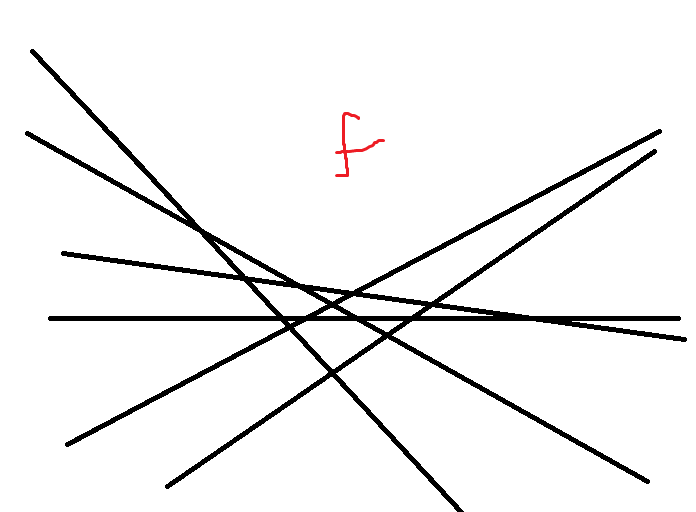
\includegraphics[scale = 0.25]{3_1_a.png}
            \caption{3.a}
        \end{figure}

        \item $(+1, 0, 0, -1, -1, -1)$
        \begin{figure}[H]
            \centering
            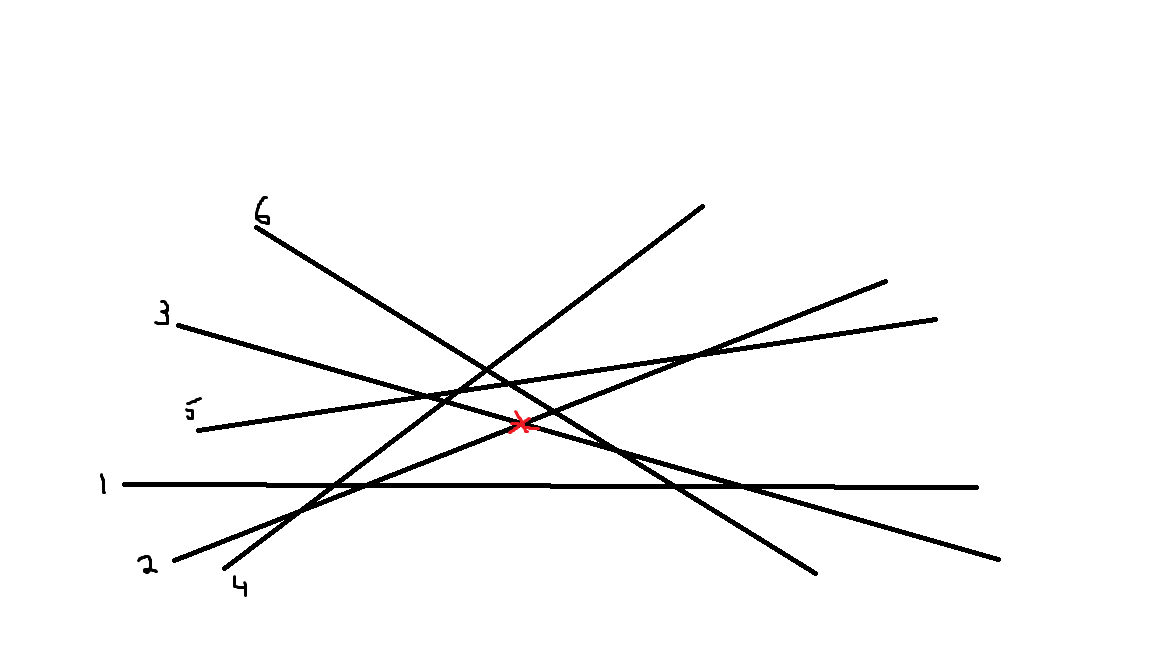
\includegraphics[scale = 0.25]{3_1_b.png}
            \caption{3.b}
        \end{figure}
        \item $(-1, 0, 0, -1, +1, -1)$
        \begin{figure}[H]
            \centering
            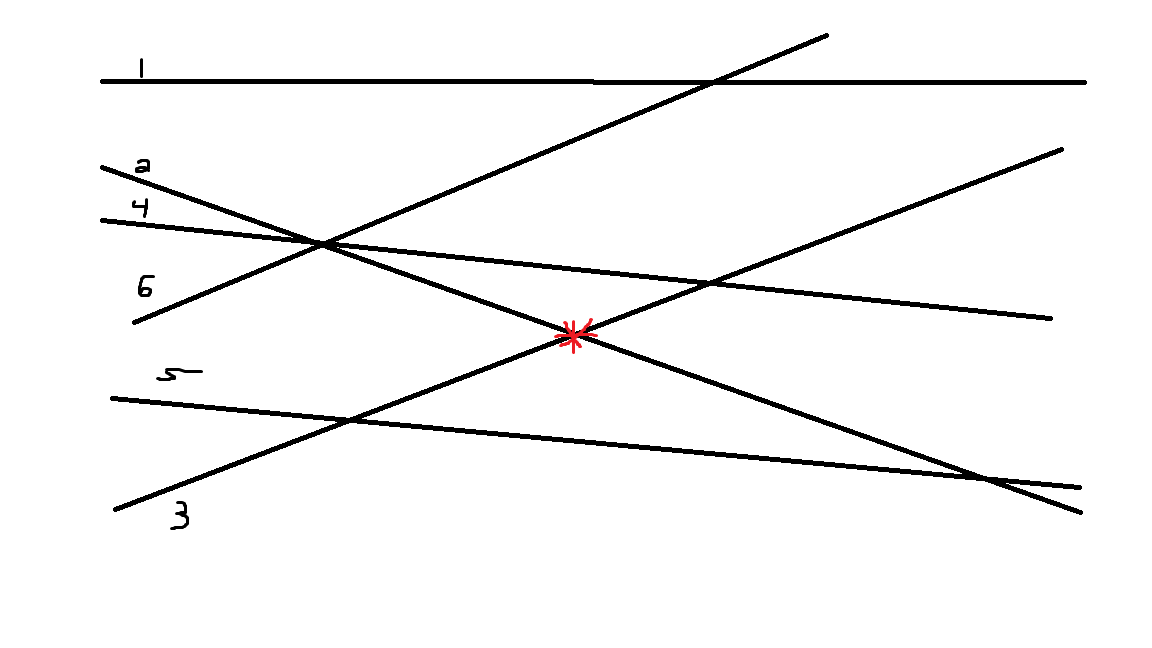
\includegraphics[scale = 0.25]{3_1_c.png}
            \caption{3.c}
        \end{figure}
        \item $(+1, -1, -1, -1, -1, -1)$
        
        \begin{figure}[H]
            \centering
            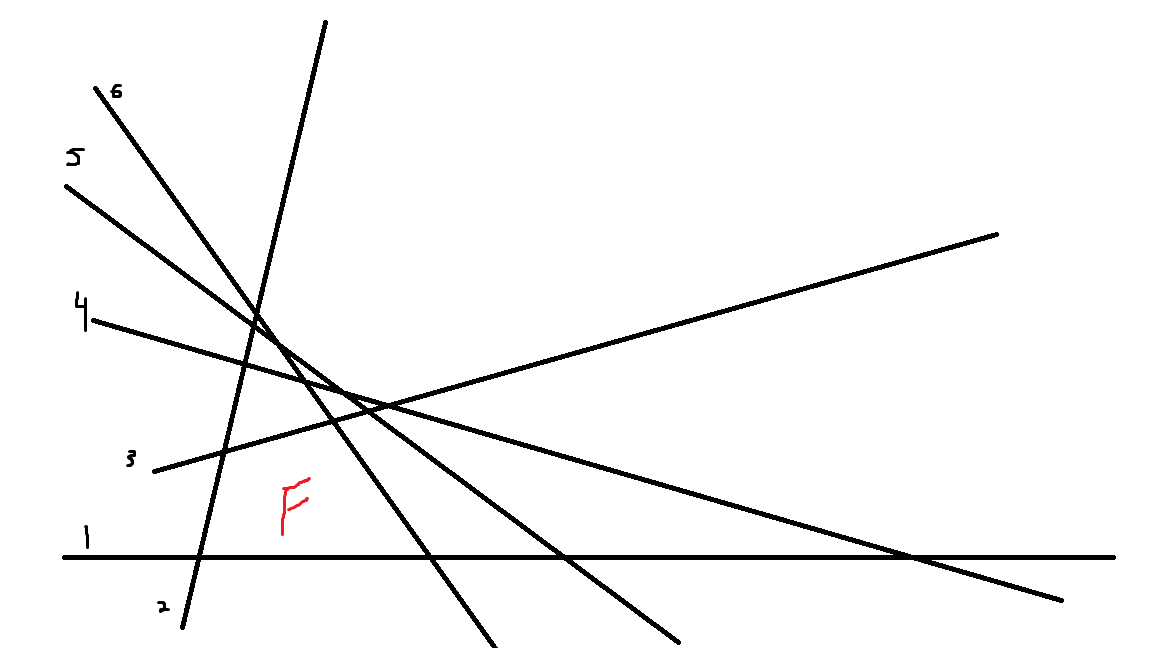
\includegraphics[scale = 0.25]{3_1_d.png}
            \caption{3.d}
        \end{figure}

    \end{enumerate}

    \item No it is not possible. Consider (b) and (c). To lie on 2 things it must be a vertex.
    For (b) vertex must be above line 1, and for (c) it has to be below line 1. Contradiction.
\end{enumerate}








\problem{4}

We saw in class a few applications of arrangements for solving geometric
problems. Find a problem whose solution was not described in class.  Give a
description of the problem and how one can use arrangements to solve the
problem.

You MAY (but do not need to) answer these questions by researching on the
internet. Cite the sources you were using and give an explanation in your own
words

\hrule


So I don't know how much of a real-world application this is. But imagine we are in a spy movie
and we are trying to guard a room so nobody can get in without setting off the alarm. 
We don't want a grid because that is too easy, but we want to make sure our lasers
don't have holes big enough for someone to fit through. 

So the lines are the lasers (plus ones for the door frame). We compute the arrangement. We compute the area by triangulating each face.
Since each face is convex we can just draw a line from one vertex to all the others to triangulate it
and then sum the area of the triangles. We want to find the face with the maximum area. 

This takes $O(n^2)$ to produce the arrangement. Then there are $O(n^2)$ faces with $O(1)$ vertices
around each face (on average, since if there wasn't there would be $O(n^3)$ vertices which isn't true by Euler's theorem),
so it takes quadratic time to compute all of the areas. So it is $O(n^2)$ alg.

More realistically this can be used to find max/min area within regions bounded by lines. 


\end{document}